\documentclass{minimal}
\usepackage[letterpaper,margin=1cm]{geometry}
\usepackage{pgfplots}
\pgfplotsset{compat=1.16}

\begin{document}
\centering
\begin{tikzpicture}[trim axis left]
  \begin{semilogyaxis}[
      width=\textwidth, scale only axis,
      height=0.85\textheight,
      % Grid
      grid=both,
      grid style={black,line width=0.12pt},
      major grid style={line width=0.24pt},
      ticks=both,
      tick style={black},
      tick label style={color=lightgray},
      % X axis
      xmin=0,
      xmax=26,
      xtick={0,...,26},
      minor x tick num=5,
      xticklabel=\empty,
      % Y axis
      ymin=20,
      ymax=80,
      ytick={20,...,40,42,44,...,80},
      yticklabels={20,...,40,42,44,...,80},
      minor ytick={20,20.25,...,40,40.5,41,...,80},
      minor y tick num=3,
    ]
  \end{semilogyaxis}
\end{tikzpicture}
\\
\begin{tikzpicture}[trim axis left]
  \begin{axis}[
      width=\textwidth, scale only axis,
      height=0.1\textheight,
      % Grid
      grid=both,
      grid style={black,line width=0.12pt},
      major grid style={line width=0.24pt},
      ticks=none,
      tick style={black},
      xmajorticks=true,
      xtick pos=lower,
      xtick align=outside,
      major tick length=10pt,
      % X axis
      xmin=0,
      xmax=26,
      xtick={0,...,26},
      xticklabel=\empty,
      minor x tick num=5,
      % Y axis
      ymin=0,
      ymax=6,
      ytick={0,...,6},
      yticklabel=\empty,
]
  \end{axis}
\end{tikzpicture}
\end{document}
